%%%%%%%%%%%%%%%%%%%%%%%%%%%%%%%%%%%%%%%%%
% University Assignment Title Page 
% LaTeX Template
% Version 1.0 (27/12/12)
%
% This template has been downloaded from:
% http://www.LaTeXTemplates.com
%
% Original author:
% WikiBooks (http://en.wikibooks.org/wiki/LaTeX/Title_Creation)
%
% License:
% CC BY-NC-SA 3.0 (http://creativecommons.org/licenses/by-nc-sa/3.0/)
% 
% Instructions for using this template:
% This title page is capable of being compiled as is. This is not useful for 
% including it in another document. To do this, you have two options: 
%
% 1) Copy/paste everything between \begin{document} and \end{document} 
% starting at \begin{titlepage} and paste this into another LaTeX file where you 
% want your title page.
% OR
% 2) Remove everything outside the \begin{titlepage} and \end{titlepage} and 
% move this file to the same directory as the LaTeX file you wish to add it to. 
% Then add \input{./title_page_1.tex} to your LaTeX file where you want your
% title page.
%
%%%%%%%%%%%%%%%%%%%%%%%%%%%%%%%%%%%%%%%%%
%\title{Title page with logo}
%----------------------------------------------------------------------------------------
%	PACKAGES AND OTHER DOCUMENT CONFIGURATIONS
%----------------------------------------------------------------------------------------

\documentclass[12pt]{article}
\usepackage[english]{babel}
\usepackage[utf8]{inputenc}
\usepackage{amsmath}
\usepackage{graphicx}
\usepackage[colorinlistoftodos]{todonotes}
\usepackage{titlesec}
\usepackage{float}
\usepackage{multicol}

%to include references in toc
\usepackage[nottoc,numbib]{tocbibind}
%bibliography package
\usepackage[backend=bibtex,style=nature,block=ragged]{biblatex}

% \usepackage{url}
% \def\UrlBreaks{\do\/\do-}
% \usepackage{breakurl}
% \usepackage[breaklinks]{hyperref}
%----------------------------------------------------------------------------------------
%	BIBLIOGRAPHY
%----------------------------------------------------------------------------------------
% \usepackage[
% backend=biber,
% style=nature,
% ]{biblatex}
% \addbibresource{ThesisProposal.bib}
% \bibliographystyle{nature}
\bibliography{ThesisProposal.bib}

\begin{document}

\begin{titlepage}

\newcommand{\HRule}{\rule{\linewidth}{0.5mm}} % Defines a new command for the horizontal lines, change thickness here

\center % Center everything on the page



 
%----------------------------------------------------------------------------------------
%	HEADING SECTIONS
%----------------------------------------------------------------------------------------

\includegraphics[width=0.3\columnwidth]{University_of_Los_Andes_logo.png}\\[1cm] %
\textsc{\Large Universidad de los Andes}\\[1.5cm] % Name of your university/college
\textsc{\large Undergraduate Thesis Proposal}\\[0.5cm] % Major heading such as course name
% \textsc{\large Minor Heading}\\[0.5cm] % Minor heading such as course title

%----------------------------------------------------------------------------------------
%	TITLE SECTION
%----------------------------------------------------------------------------------------

\HRule \\[0.4cm]
{ \Large \bfseries Transient object classification using machine learning and deep learning techniques on real data}\\[0.4cm] % Title of your document
\HRule \\[1.5cm]
 
%----------------------------------------------------------------------------------------
%	AUTHOR SECTION
%----------------------------------------------------------------------------------------

\begin{minipage}{0.4\textwidth}
\begin{flushleft} \large
\emph{Author:}\\
Mauricio Neira % Your name
\end{flushleft}
\end{minipage}
~
\begin{minipage}{0.5\textwidth}
\begin{flushright} \large
\emph{Supervisor:} \\
Marcela Hernández Hoyos, Ph.D. % Supervisor's Name
\end{flushright}
\end{minipage}\\[2cm]

% If you don't want a supervisor, uncomment the two lines below and remove the section above
%\Large \emph{Author:}\\
%John \textsc{Smith}\\[3cm] % Your name

%----------------------------------------------------------------------------------------
%	DATE SECTION
%----------------------------------------------------------------------------------------

{\large \today}\\[2cm] % Date, change the \today to a set date if you want to be precise

%----------------------------------------------------------------------------------------
%	LOGO SECTION
%----------------------------------------------------------------------------------------

\tableofcontents
 
%----------------------------------------------------------------------------------------

\vfill % Fill the rest of the page with whitespace

\end{titlepage}


\section{Introduction}

This project focuses on automatic transient object detection. This section will briefly outline the basic concepts needed to understand the motivation and reasoning behind it. 

\subsection{Astronomy}

Astronomy is the field of science that studies celestial objects i.e. starts, planets, matter, etc. Outside of earth. These objects emit electromagnetic radiation all across the electromagnetic spectrum. Measurements of this radiation have been made with a  wide variety of instruments and a lot of data has been recorded. \\

Usually, the data is recorded in \textit{surveys} where various telescopes scan the sky through many days. Of of these surveys is the subject of this papers investigation known as the ``Catalina Real Time Survey''\cite{catalina}. In this database, the intensity of radiation of various objects was recorded at different time intervals. The group of points collected for a particular object is known as a light curve.\\

\subsubsection{Light curves}

After recording the intensity of emitted radiation of an object several times, it is possible to plot the result in a scatterplot. The following image is an example of a light curve of a type 1a supernova:

\begin{figure}[H]
  \centering
  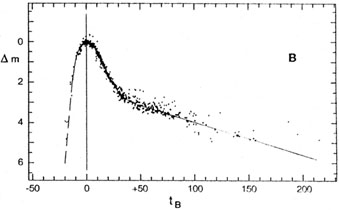
\includegraphics[width=0.8\textwidth]{snlightcurve.jpeg}c
  \caption{Light curve for a supernova type 1a \cite{snlightcurve}.}
\end{figure}

Light curves hold a lot of information about the behavior of the object and can be used to identify the type of object \cite{lc1,lc2}. A big part of this project is dedicated to classifying objects based on their light curve. 

\subsubsection{Supernovae}

Supernovae, specially type 1a supernovae, are of immense importance in present day astrophysics. They are used as ``standard candles''\footnote{A standard candle is a celestial object whose properties are optimal to measure large distances in the universe with high precision. } to estimate the rate of expansion of the universe \cite{expansion}. So far, they have been used to pin down the cosmological constant (also known as Hubble's constant) and demonstrate the accelerating expansion of the universe. This has had a huge impact on our understanding of the universe. Particularly because it ``impl[ies] the existence of a nearly uniform component of dark energy''\cite{darkEnergy} across space. \\

Finding and studying supernovae not only sheds light into their nature, it has implications that stretch out to the inner workings of the universe.

\subsection{LSST}

The Large Synoptic Survey Telescope is a project that will begin operating in 2020 and has four main goals\cite{LSST}: 

\begin{enumerate}
  \item Probing dark energy and dark matter
  \item Taking an inventory of the Solar System
  \item Exploring the transient optical sky
  \item Mapping the Milky Way
\end{enumerate}

Unlike other telescopes of its nature, from the moment it begins operation, the LSST will release its data to the public. It plans on gathering 15 terabytes of data every night, generating alerts and transferring data with a 60 second delay \cite{LSST}.\\

With that amount of data, there simply aren't enough experts to classify all of the objects of interest. New automated techniques are needed to correctly classify all of the observed objects and notify the corresponding interested scientists.Consequently, the motive behind this project is to develop an automatic classifier of astronomical objects. \\

\section{Problem description}

As stated in the previous section, the motivation behind this project is to create an algorithm that automates the classification of astronomical objects. The classification can be done directly on the images released by the CSS \cite{catalina} or on the light curves extracted from the images. 


\subsection{Classification of transient objects from light curves}

One of the main aims to develop an algorithm that correctly maps the light curve of an object to its corresponding category. It is unrealistic to claim that the function will correctly classify every single light curve it is provided. Nevertheless, it does aim to minimize classification errors. \\

There will be 2 main approaches to achieve this goal. The first will be to transfer the light curves into a feature space that attempts to extract many geometric properties of the light curves. After that, several classifiers will be applied over the data points in the feature space. These include random forests and feed forward neural networks.\\

The second approach involves feeding the points to a recurrent neural network that will in turn be fed into a feed forward neural network. 

\subsection{Classification of transient objects from images}

The second main aim of this proposed thesis is to develop an algorithm that correctly classifies astronomical objects from a series of \textit{images}. \\

In brief, the aim is to implement a convolutional neural network that extracts descriptors from the images. Following this procedure, the extracted descriptors will be fed into a recurrent neural network that will have a fully connected layer attached at the end. The output of this architecture will be an $n$ dimension vector corresponding to the $n$ classes that the astronomical object can belong to. See section \ref{NNarchitecture} for further details.\\

\section{Project Background}

\subsection{Diego's thesis - 2018-10}

In the first semester of 2018, Diego Alejandro G\'omez Mosquera worked on ``Astronomical transient event recognition with machine learning'' using a variety of traditional machine learning classifiers on a feature space calculated from light curves \cite{diegoThesis}.\\ 

The author focused on creating a feature space robust enough to distinguish the different transient classes. This was achieved primarily through geometric parameters that were extracted from the light curves. The features used and their importance during classification (as found on the author's thesis) for 8-class classification were: 

\begin{figure}[H]
  \centering
  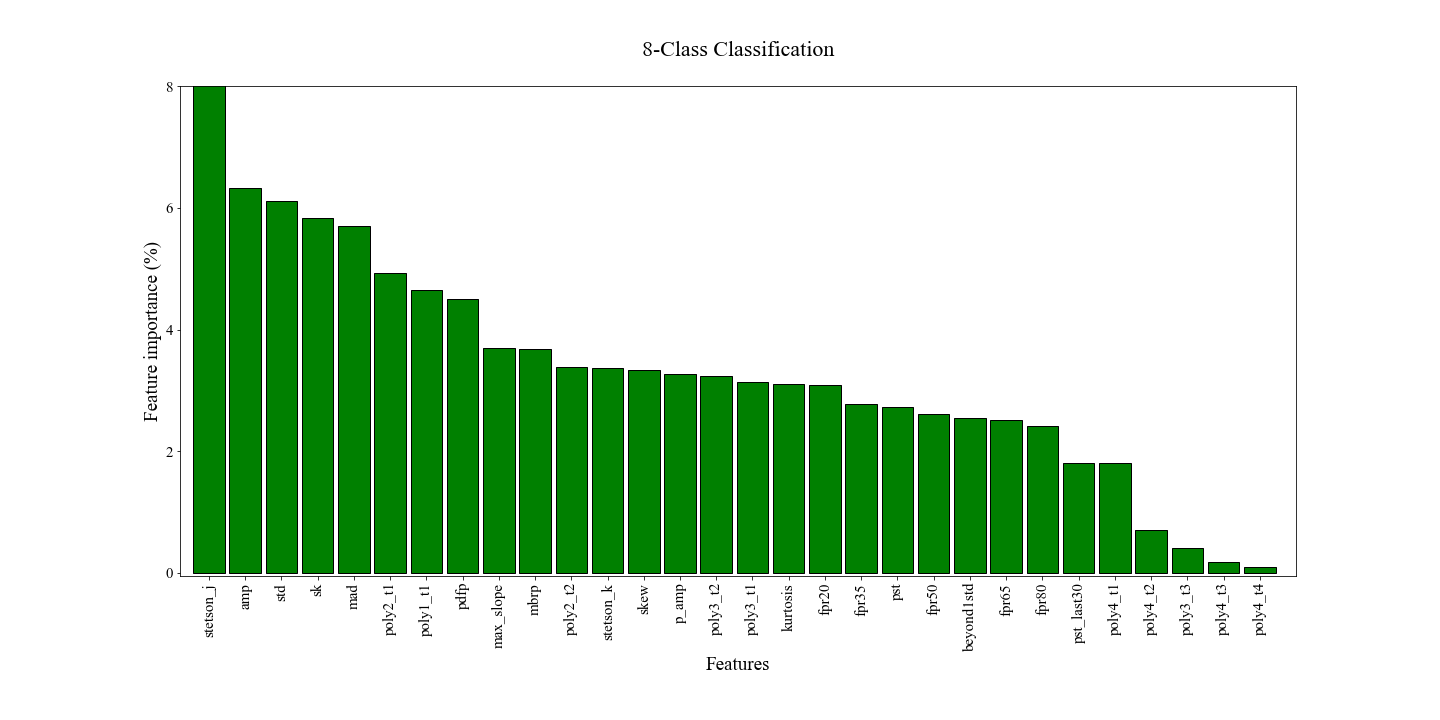
\includegraphics[width=1.05\textwidth]{images/importances.png}
  \caption{Feature importance when classifying light curves into 8 classes.}
\end{figure}

Out of all of the classifiers used, the classifier with the best results was the random forest classifier. 

The results from the authors thesis will not be presented here as a bug overrating the classification was found as will be discussed in the following section.

\subsection{research internship?? No se como ponerle a esto 2018-2}

\subsubsection{Improvement on Diego's work}\label{improvementDiego}
Diego's work was continued and improved during this semester with the mentorship of Marcela Hern\'andez, Jaime Forero and Pablo Arbelaez. 

\subsubsection{PLAsTiCC - Kaggle competition}


\section{General objective}
\section{Specific objectives}

\subsection{Improvement of the light curve feature space}

\subsubsection{Feature pruning}

After seeing the results in \ref{improvementDiego}, \textbf{REVISAR ESTO}, it was clear that the higher order coefficients in the polynomial fits did not contribute significantly to the correct classification in the feature space. In fact, these features could be harming the classification process. Thus, coefficients resulting from $3^{rd}$ and $4^{th}$ degree polynomial fitting will be removed and the random forest algorithm will be rerun. The classification metrics should improve but experimentation is needed to confirm the hypothesis.  

\subsubsection{Addition of supernovae specific metrics}

To improve the classification of supernovae, metrics that target their specific light curve behavior are needed. In particular, there are functions that are known to approximate the light curve produced by a supernova. These functions are presented below: 

\paragraph{SALT2} is ``an empirical model of Type Ia supernovae spectro-photometric evolution with time''\cite{salt2}. This model should be better adjusted for type 1A supernovas than the rest of objects. The mathematical model of the function is the following\cite{salt2}:

\[
  F(S,N,p,\lambda) = x_0 \times [M_0(p,\lambda)+x_1M_1(p,\lambda)+...]\times exp[cCL(\lambda)]
\]

\paragraph{Skewed Gaussian} fits of the form:

\[f^k(t) = A^k \frac{exp-(t-t_0^k/\tau^k_{fall})}{1+exp-(t-t^k_0)\tau^k_{rise}}\]

have been shown to resemble well a generalized supernova curve \cite{sGaussian}. It should also approximate the shape of supernova light curves better than those that belong to other classes.\\

When these functions are fit to supernovae data, the resulting $\chi^2$ should be considerably lower than the $\chi^2$ calculated from non-supernovae fits. Consequently, the addition of the two $\chi^2$  values from each of the functions should improve the binary classification of supernovae but as stated above, experimentation is needed for verification.

\subsection{Deep learning on light curves}

For the time being, the classification pipeline has had 3 steps:

\begin{enumerate}
  \item Clean and filter light curves
  \item Calculate features from clean light curves
  \item Classify the objects on the feature space
\end{enumerate}

When the feature space is calculated, a large quantity of information is lost. The features might be good descriptors of the objects but they will never be able to encapsulate the point-by-point data that the light curves have. Additionally, traditional machine learning methods, like the random forest classifier previously implemented, are unable to handle varying length input. To take advantage of all the information present in the light curves, a new approach is needed.\\

Recurrent neural networks (RNN) have been shown to be able to classify sequential data to a good extent. Speech recognition has been one of the fields with most progress\cite{RNN}. A RNN like the long short term memory (LSTM) RNN or the gated recurrent unit (GRU) RNN are state of the art RNN's that seem promising for this purpose. Thus, several implementations of these networks will be carried out along with their hyperparameter tuning. 

\subsection{Deep learning on images}

\subsubsection{CNNs}

So far, all the classification has been done on the objects' photometric light curves. The light curves, however, are not the raw data. These were calculated from the images that were taken by the telescopes. Specifically, the light curves werre calculated from the catalina real time survey images \cite{catalinaImages}. Ideally, to minimize data loss, the classification process should be done on the raw data i.e. the images.\\ 

The state of the art algorithms used for classifying images are known as convolutional neural networks (CNNs) \cite{CNN} and have had wide success on large variety of problems.\\

The first step to correctly classify the images will be to implement a baseline CNN algorithm. Once its classification  metrics are established, a thorough search through the hyperparameter space will be carried out to maximize the classification metrics.

\subsubsection{CNNs and RNNs}\label{NNarchitecture}

Implementing a succesful CNN is only half of the problem. Each object has multiple images taken at different instances in time. To fully exploit the available information, multiple images need to be used as input for each object.\\

Since the amount of images per object is not fixed, a RNN will need to be used. Thus, the CNN will extract descriptors from the images and then those descriptors will be fed in chronological order along with the date of when the image was taken into the RNN for classification. The architecture is depicted below:

\begin{figure}[H]
  \centering
  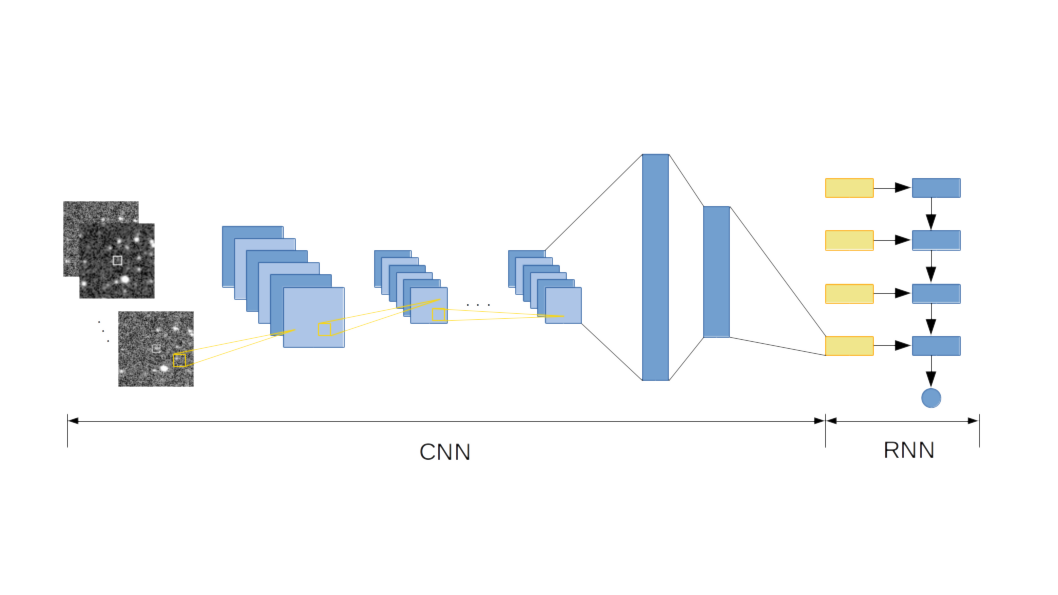
\includegraphics[width=1.05\textwidth]{CNNRNNDiagram.png}
  \caption{Architecture for classifying astronomical objects from multiple images.}
\end{figure}

\section{Activities and schedule}


\section{Expected results}


\newpage
\printbibliography

\end{document}